\subsection{Data collector}
	La componente \textit{data collector} permette di trasferire i dati prodotti dai singoli gateway ed inviati nei vari topic di Kafka, all'interno di un database di tipo timeseries.
	\newline
	Allo stesso tempo, permette di filtrare i dati collezionati ed inviare dei messaggi di avviso, all'interno di un apposito topic, nel caso in cui vengano rilevati dei valori anomali.
	\newline
	Il filtraggio dei dati viene fatto a partire dagli alert impostati all'interno della web app e salvati in un database relazionale (PostgreSQL).
	\begin{itemize}
		\item La componente è stata sviluppata in Java 11.
	\end{itemize}
	
		\subsubsection{Diagramma dei package}%%%%%%%%%OK
		\begin{figure}[H]
				\centering
				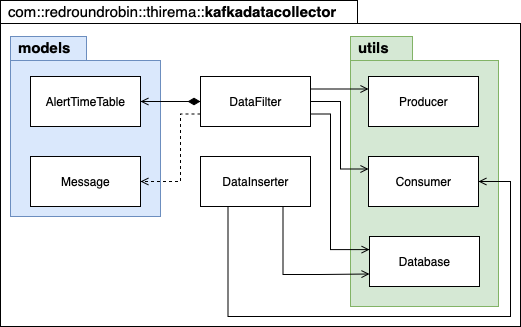
\includegraphics[scale=0.600]{res/images/DATACOLLECTOR/Packagekafkadatacollector.png}
				\caption{Diagramma dei package della componente data collector}
				\label{Diagramma 5}
			\end{figure}
		\begin{landscape}
		\subsubsection{Diagramma delle classi}%%%%%%%%%%%%%%%%%%%%%%%OK
			\begin{figure}[H]
				\centering
				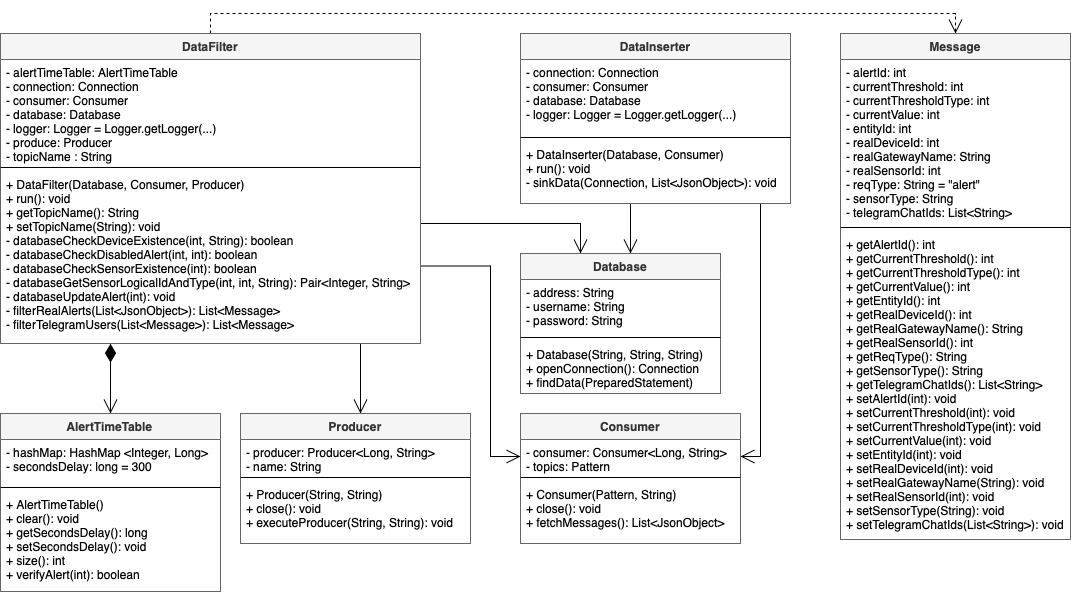
\includegraphics[scale=0.550]{res/images/DATACOLLECTOR/ClassikafkaDataCollector.png}
				\caption{Diagramma delle classi della componente data collector}
				\label{Diagramma 6}
			\end{figure}
		\end{landscape}
		\begin{landscape}
		\subsubsection{Diagrammi di sequenza}%%%%%%%%%OK
			\begin{figure}[H]
				\centering
				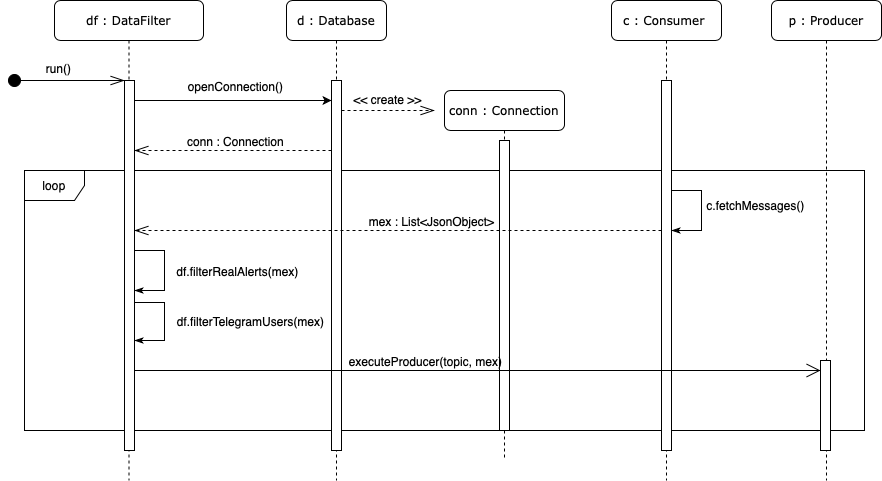
\includegraphics[scale=0.550]{res/images/DATACOLLECTOR/DataFilter.ThreadsKafkaDataCollector.png}
				\caption{Diagramma di sequenza in cui viene mostrato il funzionamento del filtraggio dati nella componente data collector}
				\label{Diagramma 7}
			\end{figure}
			\begin{figure}[H]
				\centering
				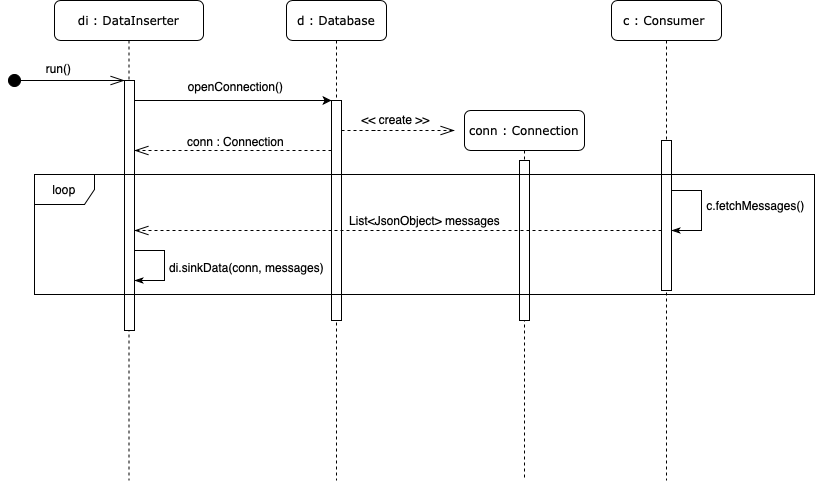
\includegraphics[scale=0.550]{res/images/DATACOLLECTOR/DataInserter.ThreadsKafkaDataCollector.png}
				\caption{Diagramma di sequenza in cui viene mostrato il funzionamento dell'inserimento dati nella componente data collector}
				\label{Diagramma 8}
			\end{figure}
	\end{landscape}